\Chapter{JavaScript implementáció}

% Kb. 8-12 oldal

\Section{A p5 függvénykönyvtár}

% Fél-egy oldalas áttekintés a p5-ről.

\Section{Az alkalmazás felépítése}

% Blokkdiagram féle, hogy mi hol helyezkedik el az alkalmazásban.

\Section{Definiált osztályok bemutatása}

% UML osztálydiagram.
% Minden osztályról érdemes legalább 1-2 mondatot írni.
% A megvalósítással kapcsolatos tapasztalatokat is lehet itt részletezni.

\begin{figure}[!h]
	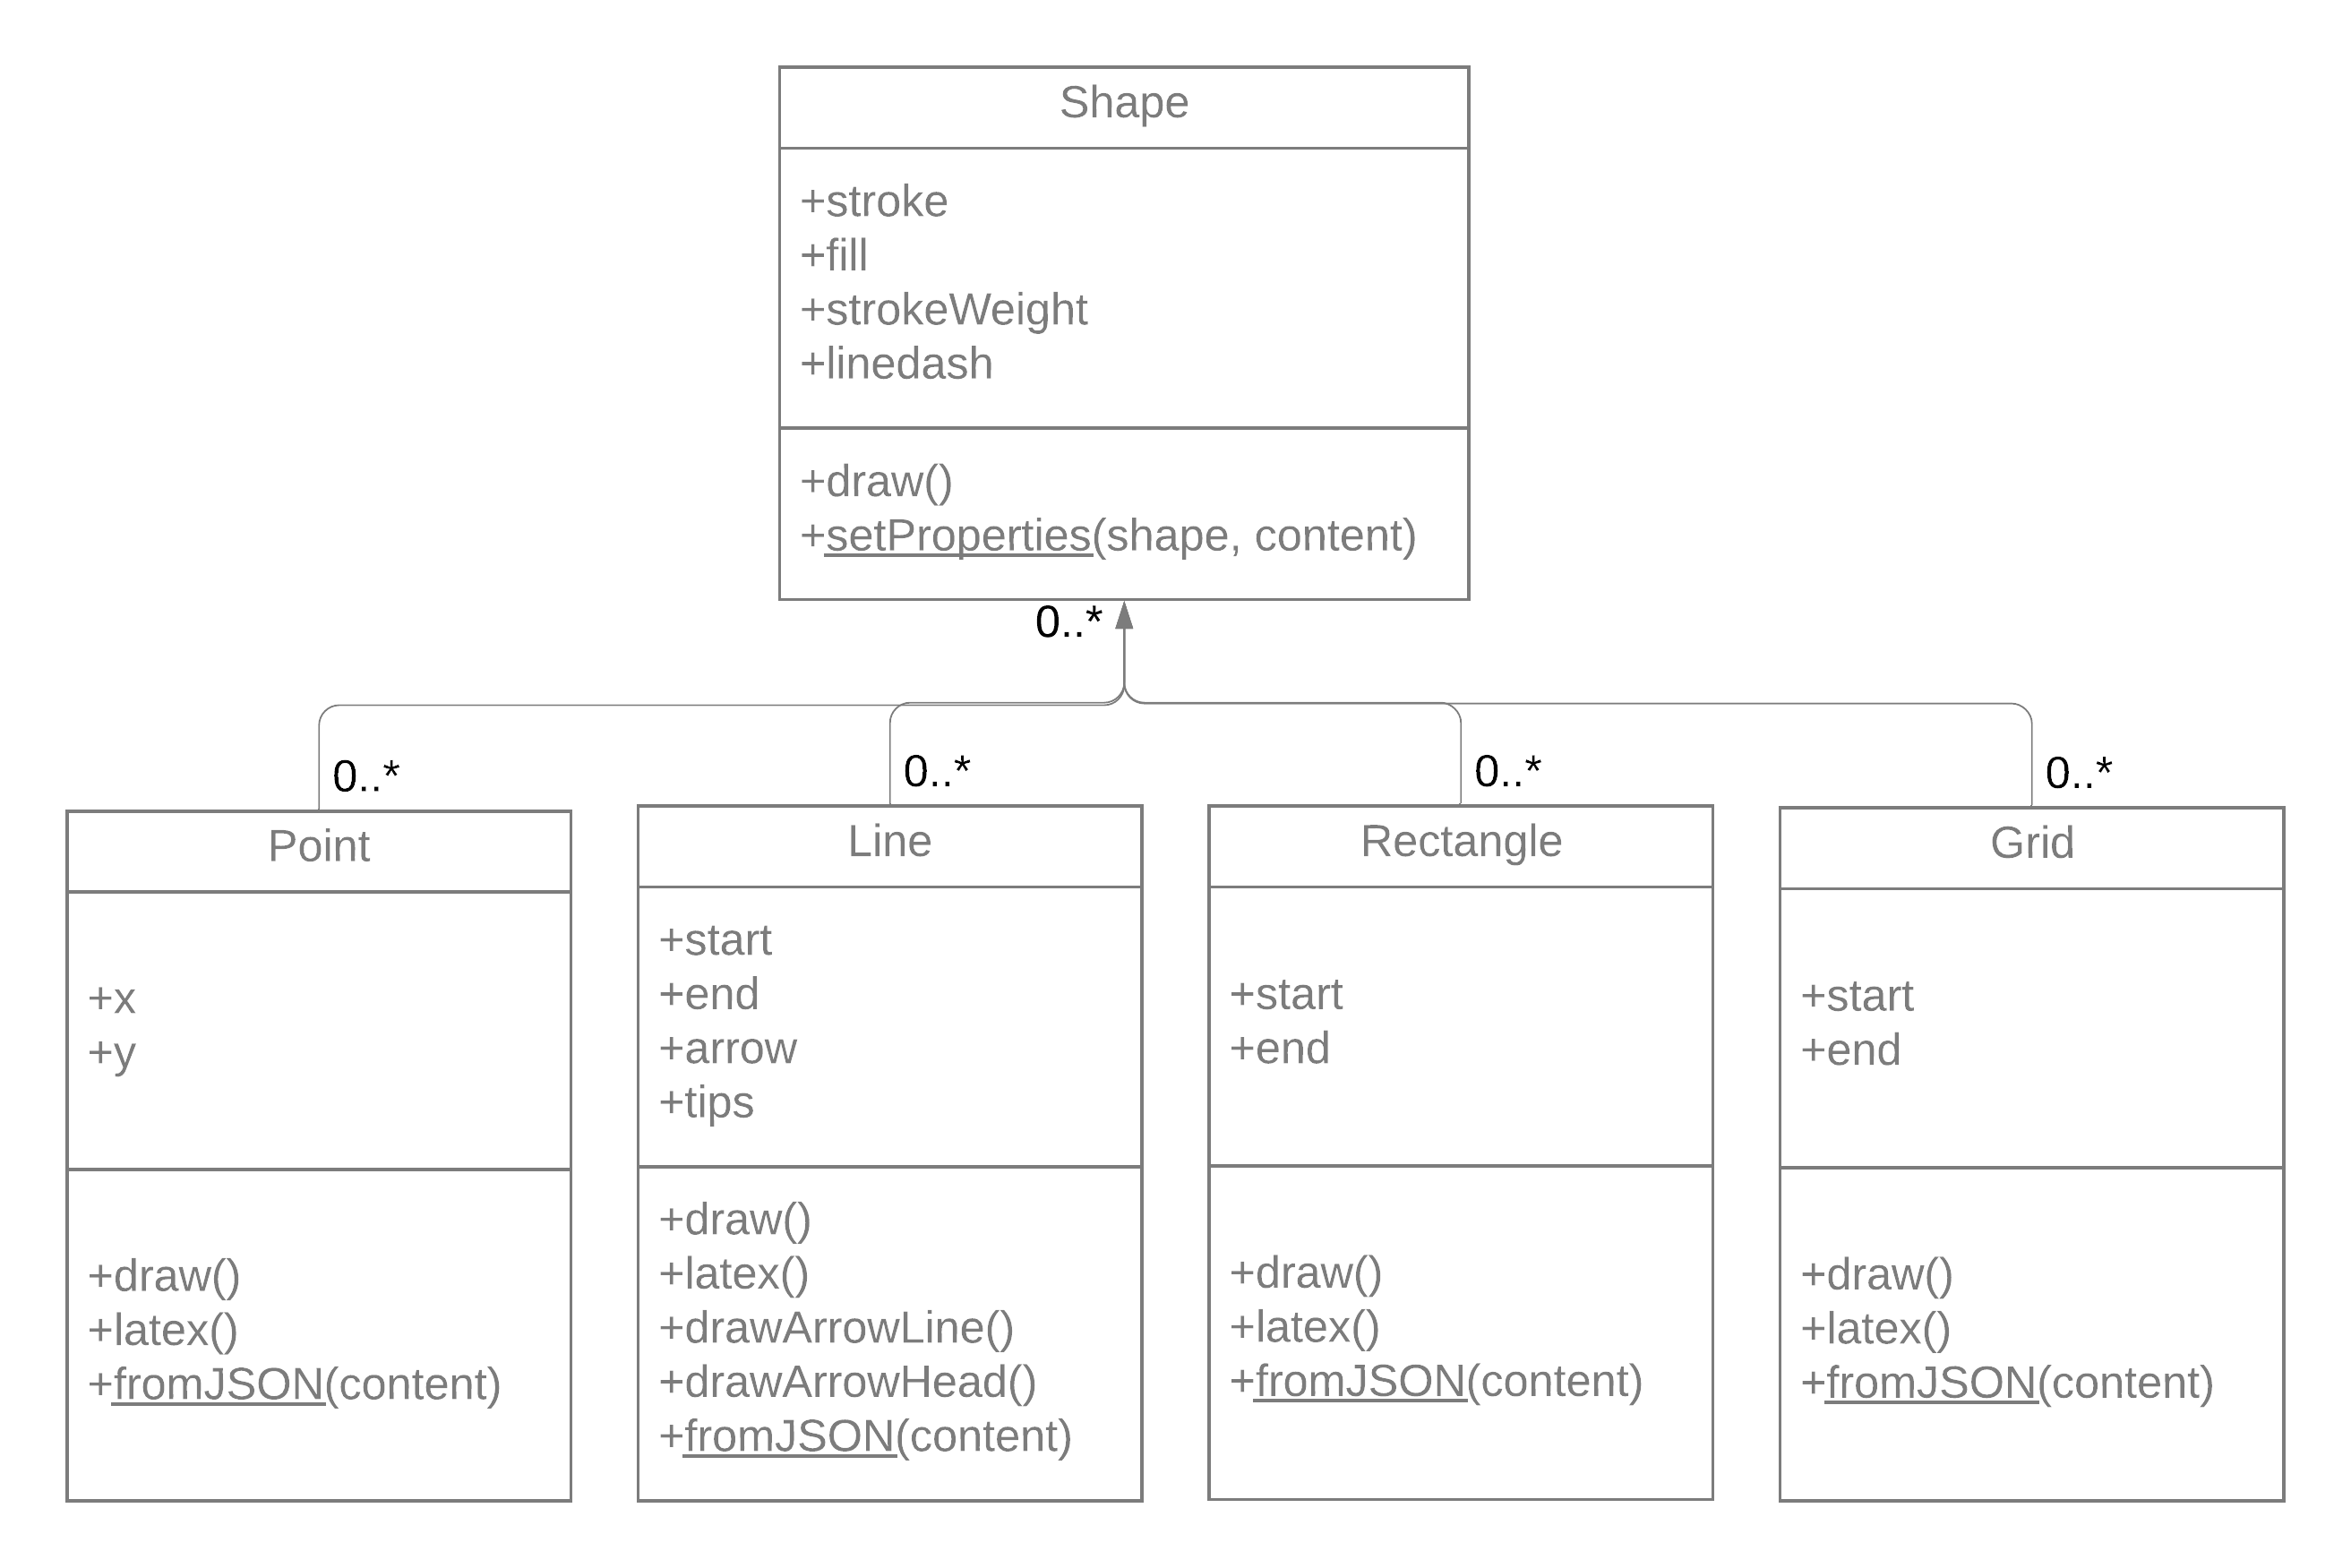
\includegraphics[width=\textwidth]{images/uml1.png}
	\caption{Az osztályok UML diagrammja (1)}
	\label{fig:uml1}
\end{figure}

\begin{figure}[!h]
	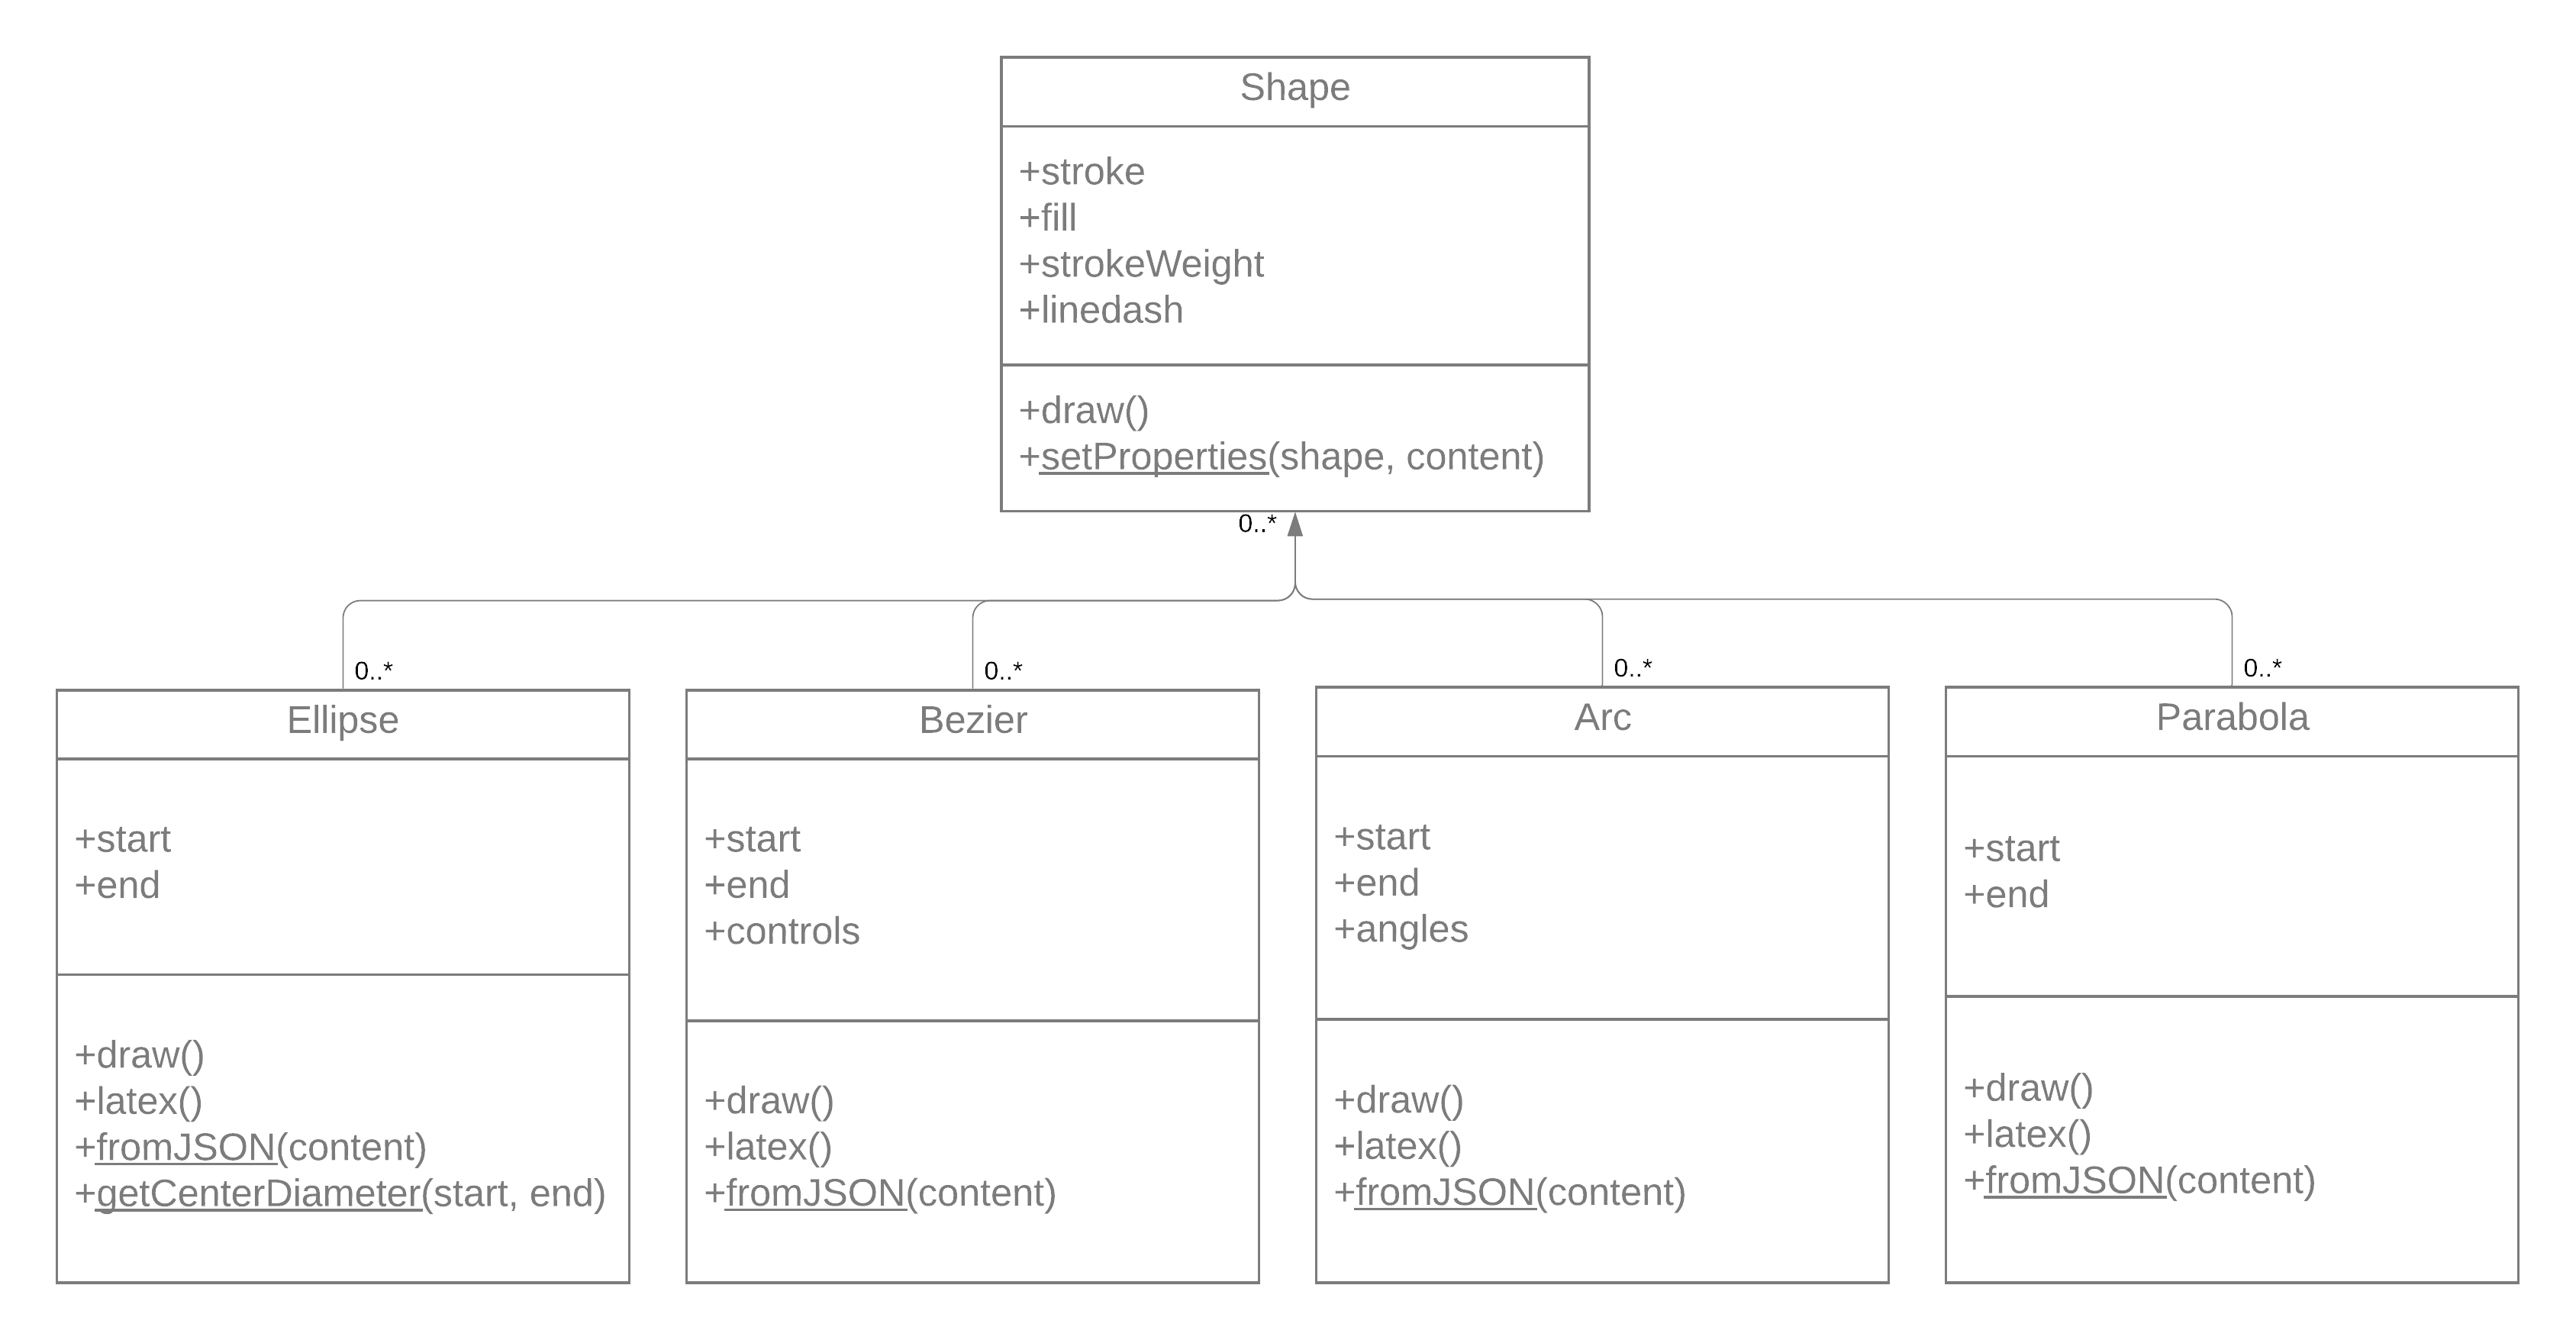
\includegraphics[width=\textwidth]{images/uml2.png}
	\caption{Az osztályok UML diagrammja (2)}
	\label{fig:uml2}
\end{figure}

